\chapter{Apéndice A: Minería de Datos}
En el capitulo anterior señalamos las diferentes alternativas que se tienen para lograr nuestros objetivos. A continuación, y en base al análisis anterior, se concluye que se utilizarán las siguiente metodología y marcos de trabajos.
\section{Metodología Escogida}
En base a lo observado en el capitulo anterior, se observan dos diferentes metodologías útiles: KDD y CRISP-DM. Como ya se señaló, es muy típico utilizar CRISP-DM para investigaciones.
A continuación se presenta en la Figura~\ref{fig:met} la metodología a utilizar, que básicamente es parecida a las metodologías anteriormente descritas.
\begin{figure}[H]
  \centering
    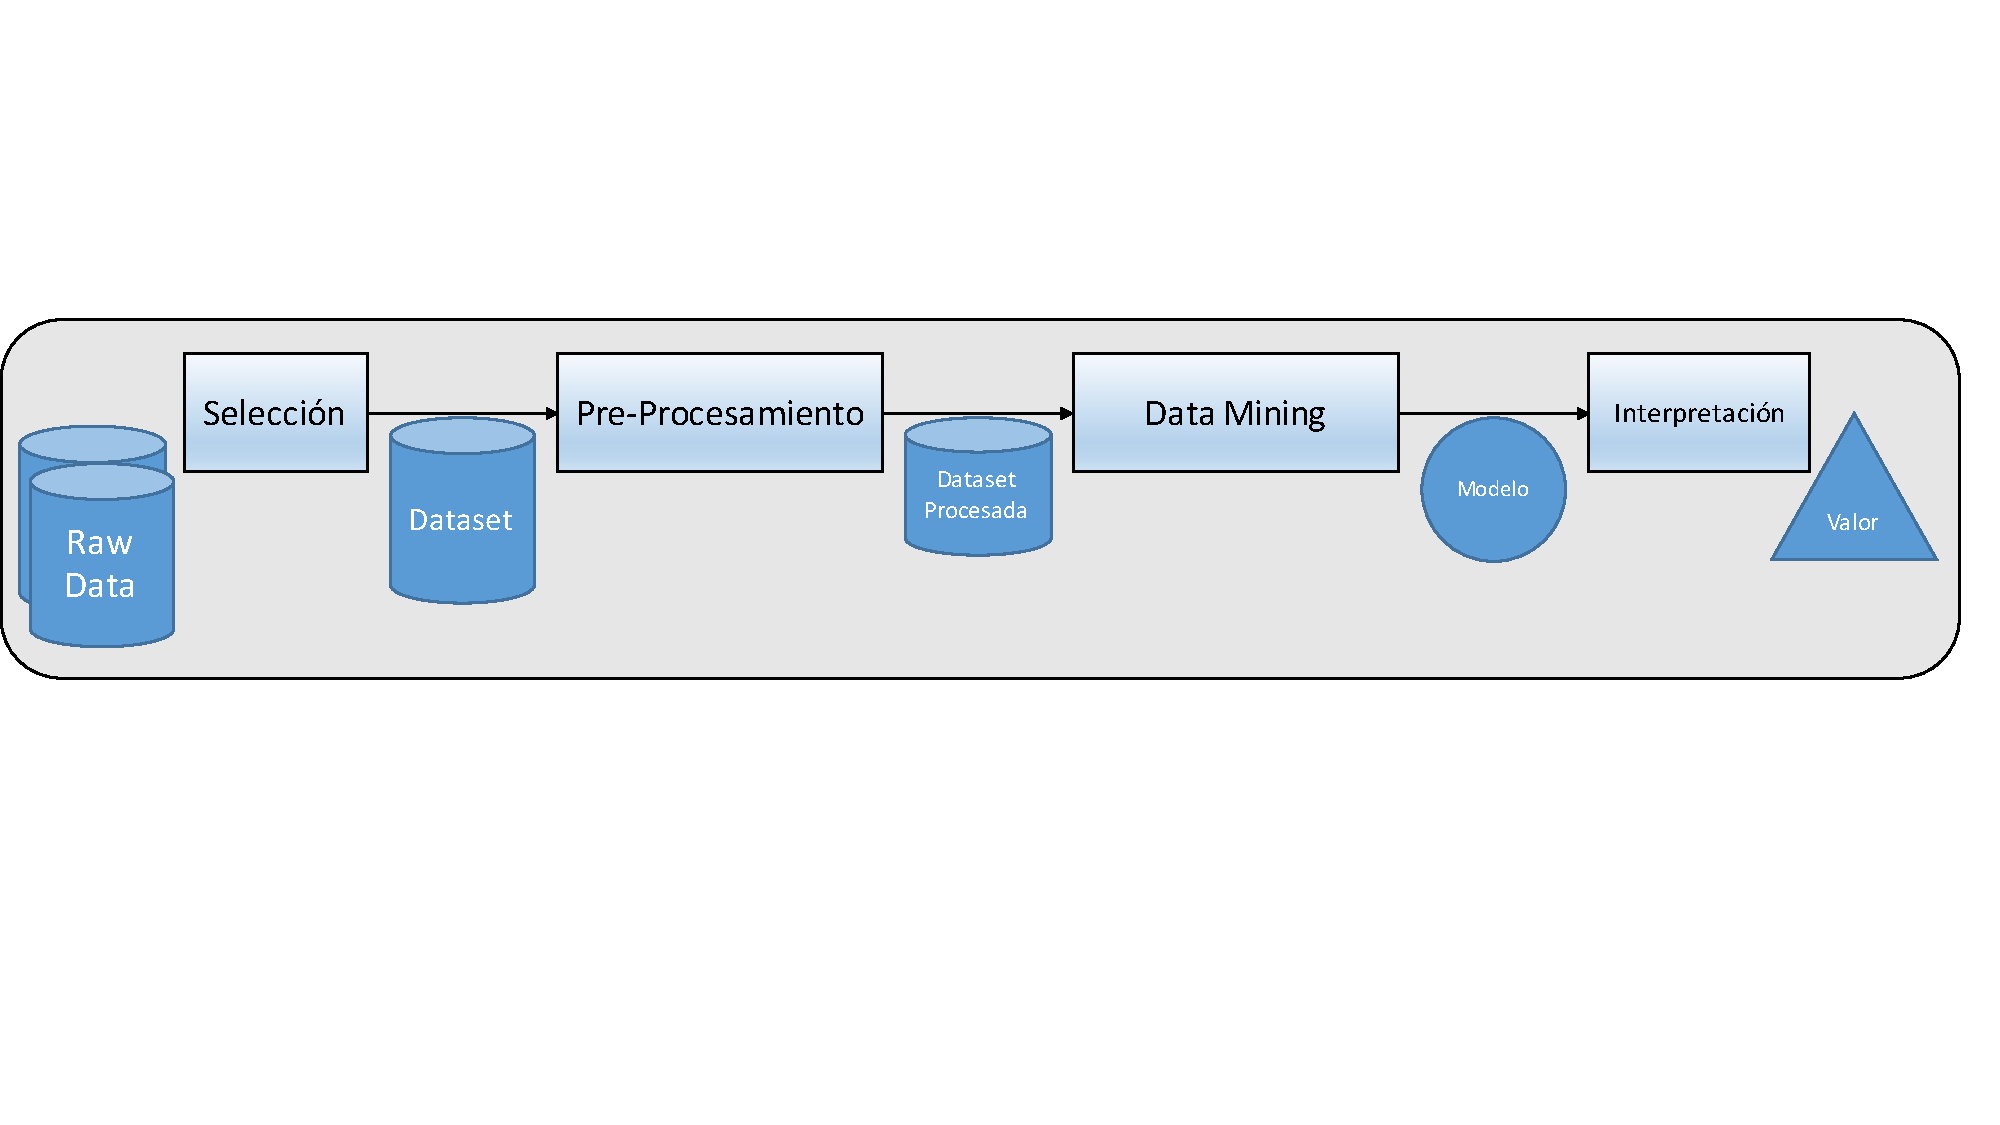
\includegraphics[width=1\textwidth]{Figuras/Metodologia}
      \caption{Proceso de \textit{Data Mining} a utilizar}
    \label{fig:met}
\end{figure}
\section{Herramientas de Minería de Datos}
Debido a que algunos de los modelos señalados en el capítulo anterior son una caja negra, no podemos saber qué tan buenos serán sin antes evaluar el desempeño de cada uno en particular. Es por esta razón que haremos una evaluación técnica de todos los algoritmos de minería de datos disponibles y en base a la métrica que señala cuántos casos son correctamente clasificados (y eventualmente usando un análisis de sensibilidad de costos de las clasificaciones). Se decidirá cuál será el algoritmo que se utilizará en la implementación.
\section{Herramientas Escogidas}
A continuación se hará una breve referencia al marco de trabajo escogido para el desarrollo del proyecto.
\subsection{Framework}
\subsubsection{Python}
Para la exploración y pre-procesamiento de la información se utilizará Python, utilizando módulos de carácter libre y con posibilidad de uso comercial. Como señalamos en el capitulo anterior, esta es la gran ventaja de Python comparado con SPSS de IBM.

Los módulos a utilizar en Python son los siguientes:
\begin{itemize}
\item scikit-learn
\item pandas
\item Numpy
\item matplotlib
\item SciPy
\end{itemize}

\subsubsection{Apache Hadoop}
Como se habló en el capitulo anterior, Apache Hadoop es útil cuando manejamos demasiada información y debemos procesarla en un solo computador, dando la posibilidad de usar $N$ computadores en paralelo. El problema de Apache Hadoop es su complejidad y las empresas que ofrecen alternativas para uso comercial, normalmente cobran el uso de sus herramientas. Por esta razón tenemos varias alternativas viables para lograr la implementación del trabajo que se deberá definir durante el mismo proyecto en base a la extensión cual es la mejor a usar. Estas son las siguientes:
\begin{itemize}
\item PredictionIO
\item MapR
\item Cloudera
\item HDP(Horton Networks)
\end{itemize}